\lecture{Lean Production e Plant Layout}{25~-~01~-~2026}
%
Questa lezione introduce i concetti base e le origini della filosofia Lean.
%
\section{Fondamenti del LEAN}
La Lean Production (Produzione Snella) non è una semplice tecnica, ma una filosofia gestionale nata in Giappone negli anni '50 con il Toyota Production System. L'obiettivo fondamentale è ``fare di più con meno'': meno risorse, meno energia, meno scarti, puntando alla sostenibilità e all'approccio di sistema. Nasce dal Toyota Production System, il termine è stato reso celebre dal libro ``The Machine That Changed the World'' (Womack, Jones, Roos, 1990).
%
\subsection{The 3'Ms}
Vengono racchiusi i 3 principi di inefficienza in 3 parole che iniziano con la ``M'':
\begin{itemize}
    \item \emph{Muda} (spreco): Tutto ciò che non aggiunge valore al prodotto. Esistono 7 tipi principali di spreco:
          \begin{enumerate}
              \item Waiting (Attesa): Tempo perso aspettando strumenti o parti.
              \item Correction (Correzione): Riparazioni o rilavorazioni.
              \item Motion (Movimento): Movimenti umani inutili (es. camminare per cercare attrezzi).
              \item Processing (Processo): Fare più lavoro del necessario.
              \item Inventory (Scorte): Eccesso di materie prime o prodotti finiti.
              \item Overproduction (Sovrapproduzione): Produrre più del necessario o prima del necessario.
              \item Conveyance (Trasporto): Trasporto inutile di materiali.
          \end{enumerate}
    \item \emph{Mura} (inconsistenza/variabilità): Mancanza di standardizzazione che riduce l'efficienza. Henry Ford sottolineava l'importanza della standardizzazione come base per il miglioramento futuro.
    \item \emph{Muri} (irrazionalità/sovraccarico): Situazioni irragionevoli, come lamentarsi dei problemi invece di cercare soluzioni.
\end{itemize}
Lean richiede una cultura ``Non-Blaming'' (senza colpa). I problemi sono visti come opportunità e le persone non sono il problema, ma i risolutori di problemi.
%
\subsection{Metodologia chiave}
Il termine descrittivo fondamentale del LEAN è ``Kaizen'', che significa ``Miglioramento continuo''. \\
Composto da ``Kai'' (Cambiamento) e ``Zen'' (Buono). Sono iniziative per eliminare gli sprechi e aumentare la produttività attraverso piccoli passi continui.
Di seguito vediamo le metodologie chiave per la LEAN.
\subsubsection{Le 5S}
Il metodo delle 5S è una metodologia di organizzazione del posto di lavoro, è composta da:
\begin{enumerate}
    \item Sort: Separare ciò che serve da ciò che non serve.
    \item Stabilize: Ordinare efficientemente.
    \item Shine: Pulizia.
    \item Standardize: Standardizzare le procedure.
    \item Sustain: Mantenere la disciplina nel tempo.
\end{enumerate}
\subsubsection{Industria Push Pull}
\begin{itemize}
    \item \textbf{Push}: Si produce ``just in case' (per scorta), accumulando inventario tra le macchine.
    \item \textbf{Pull}: Si produce solo quando il cliente (o la fase successiva) lo richiede. Usa il Kanban (cartellino fisico che contiene informazioni) come segnale di autorizzazione.
\end{itemize}
\subsubsection{Just in time}
Il ``just in time'' è la pratica che consiste nel produrre il numero richiesto di parti, al momento giusto. Si basa sul Takt Time, il ritmo che la produzione deve seguire per soddisfare la domanda del cliente.
Questa pratica evita la sovrapproduzione di prodotti, uno dei principali sprechi e impedimenti nelle linee di produzioni industriali.
\subsubsection{Sistemi poka-yoke}
I sistemi ``poka-yoke'', che si traduce in ``a prova di stupido'', sono sistemi che rendono impossibili gli sbagli nella costruzione e produzione di un prodotto.
\begin{example}
    La SIM Card è un sistema Poka-Yoke, può essere inserita in un unico verso, con un unico orientamento.
\end{example}

%
\section{Principi del LEAN thinking}
Il pensiero LEAN si divide in 5 principi fondamentali:
\begin{enumerate}
    \item Value: Specificare il valore dal punto di vista del cliente.
    \item Value Stream: Identificare il flusso del valore ed eliminare gli sprechi.
    \item Flow: Creare un flusso continuo.
    \item Pull: Lasciare che sia il cliente a ``tirare'' la produzione.
    \item Perfection: Puntare alla perfezione (Kaizen, miglioramento infinito).
\end{enumerate}

%
\section{Strumenti operativi della Lean}
Per implementare la teoria, utilizziamo strumenti pratici specifici.
\subsection{Value Stream Mapping (VSM)}
Mappa il flusso del valore (materiali e informazioni) dallo stato attuale (Current State Map) a quello desiderato (Future State Map).
%
\paragraph{Obiettivo} Visualizzare non solo i processi, ma il valore per il cliente, evidenziando dove il flusso si interrompe (scorte, triangoli di pericolo).
%
\paragraph{Parametri chiave} Tempo ciclo (C/T), Tempo di set-up (C/O), Uptime, Lead Time e Tempo a Valore Aggiunto.

%
\subsection{5 Whys}
Tecnica investigativa per trovare la causa radice di un problema chiedendo ``perché?'' ripetutamente (indicativamente 5 volte) fino a superare le cause apparenti.

%
\subsection{Spaghetti Chart}
Tracciamento grafico dei movimenti fisici di persone e materiali su una planimetria. Serve a visualizzare il caos, gli incroci e le distanze eccessive per poi ridurle.

%
\subsection{Metodo A3}
Problem solving sintetizzato su un foglio formato A3: a sinistra l'analisi del problema attuale, a destra il piano di implementazione futuro.

%
\section{Lean Production e Layout a Isole}
Il layout a isole è considerato il cuore della Lean perché permette il flusso a pezzo singolo (o piccoli lotti), riducendo drasticamente le scorte e i tempi di attraversamento.
%
\subsection{Caratteristiche dell'Isola Ideale}
%
\paragraph{Forma a U} Facilita il bilanciamento, la comunicazione e permette a un operatore di gestire entrata e uscita.
%
\paragraph{Supermarket} Magazzini a scaffali a gravità posti tra le isole. Funzionano secondo logica FIFO (First In First Out) e servono a disaccoppiare i processi evitando la sovrapproduzione.
%
\paragraph{Automazione} Va introdotta con cautela (rischio rigidità). È utile per qualità, sicurezza o lavori pesanti, ma non deve sostituire la flessibilità dell'operatore umano.

%
\subsection{Dimensionamento dei Lotti}
Per decidere quanto produrre, si usa il metodo Every Product Every Interval (EPEI), che tende all'ideale di produrre ogni prodotto ogni giorno. La formula per calcolare l'intervallo è:
\[
    \text{EPEI} = \frac{\text{Tempo totale di setup per campagna}}{\text{Tempo disponibile al giorno}-\text{Tempo totale di run al giorno}}
\]
Dove la ``campagna'' è la sequenza ripetitiva di tutti i prodotti. Questo calcolo ci guida nel dimensionare i lotti in base alla capacità dei contenitori e al tempo disponibile.

%
\section{Processo di Re-Layout}
Come si trasforma un layout esistente in uno Lean? La procedura standard prevede:
\begin{enumerate}
    \item \textbf{Analisi AS-IS}: VSM attuale, Spaghetti Chart, analisi dei dati (domanda, tempi ciclo).
    \item \textbf{Identificazione sprechi}: Uso dei 5 Whys per capire le cause di attese e trasporti.
    \item \textbf{Progettazione TO-BE}: Applicazione 5S, ridisegno layout, creazione VSM futura.
    \item \textbf{Misurazione}: Confronto KPI (tempi, distanze, capacità).
\end{enumerate}

\begin{figure}
    \centering
    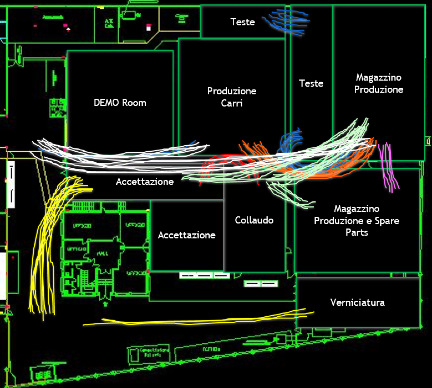
\includegraphics[width=0.5\linewidth]{assets/18.png}
    \caption{Spaghetti Chart}\label{fig:spaghetti_chart}
\end{figure}